% Pipeline figure, v5 (layout agreed in fig_pipeline_v5.drawio), drawn at final print width 16.5 cm.
% No connectors between panels: flow is carried by panel order, colour (blue = model output, dark = human data,
% vermilion = trainable theta), the repeated p_{t,k}(theta) glyph, and the panel subtitles.
% Example: Electricity task wu2025:plan_choice:p14_p36_o6, respondent wu2025_54 (code/data/base.py:make_view, include_country=False as in the paper's runs). Tokens: role names from
% code/kev/kev/model.py:encode. Backbone: Qwen3.5 block (3 Gated DeltaNet + 1 gated attention) repeated L/4 times.
% Notation follows manuscript-training.qmd: hat beta = OLS on human outcomes, bar beta(theta) = OLS on expected outcomes.
% Bars and dots are illustrative values. Equation numbers: (2) eq-resp-ce, (3) eq-pop-ols, (4) eq-eval-mse.
% Build: pdflatex fig_pipeline_v5.tex
\documentclass[tikz,border=2pt]{standalone}
% Shared look for the pipeline figures. Sizes are final print sizes (no scaling in the manuscript).
% Colors: Okabe-Ito. Blue = model prediction, vermilion = trainable theta, dark gray = human / data.
\usepackage[T1]{fontenc}
\usepackage{lmodern}
\usepackage{amsmath,amssymb,bm}
\usepackage{array}
\renewcommand{\familydefault}{\sfdefault}
\usetikzlibrary{positioning,arrows.meta,calc,fit,backgrounds}
\pgfdeclarelayer{back}\pgfsetlayers{back,background,main}

\definecolor{cpred}{HTML}{0072B2}
\definecolor{ctrain}{HTML}{D55E00}
\definecolor{chuman}{HTML}{333333}
\definecolor{cline}{HTML}{555555}
\definecolor{cfield}{HTML}{F2F2F2}
\definecolor{cframe}{HTML}{BBBBBB}
\definecolor{ctok}{HTML}{007A5A}  % Okabe-Ito bluish green, darkened: special tokens

\tikzset{
  >={Stealth[length=3.5pt]},
  every node/.append style={execute at begin node={\hyphenpenalty=10000\exhyphenpenalty=10000}},
  flow/.style={->, line width=0.6pt, draw=cline},
  pred/.style={->, line width=0.9pt, draw=cpred},
  grad/.style={->, line width=0.8pt, draw=ctrain, dash pattern=on 3pt off 2pt},
  panel/.style={draw=cframe, line width=0.5pt, rounded corners=3pt},
  ptitle/.style={font=\footnotesize\bfseries, anchor=north west, inner sep=0pt},
  raw/.style={draw=cframe, fill=white, rounded corners=1.5pt, font=\scriptsize, align=left, inner sep=2.5pt},
  field/.style={draw=cline, fill=cfield, rounded corners=1.5pt, font=\scriptsize, align=left, inner sep=2.5pt},
  box/.style={draw=cline, fill=white, rounded corners=2pt, align=center, font=\footnotesize, inner sep=2.5pt},
  predbox/.style={box, draw=cpred, line width=0.8pt},
  humanbox/.style={box, draw=chuman, line width=0.8pt},
  trainbox/.style={box, draw=ctrain, line width=0.9pt},
  rawtxt/.style={raw, draw=none, fill=none},
  fieldtxt/.style={field, draw=none, fill=none},
  note/.style={font=\scriptsize, text=black!70, align=left, inner sep=0pt, anchor=north west},
}
\newcommand{\tok}[1]{\textcolor{ctok}{\textbf{\texttt{#1}}}}
% \rowboxes{raw node}{field node}{bottom coordinate}: draws both boxes down to the lower of the two bottoms,
% so a raw item and its input field always have the same height, and links them with an arrow at mid-height.
\newcommand{\rowboxes}[3]{%
  \path let \p1=(#1.south), \p2=(#2.south), \n1={min(\y1,\y2)} in coordinate (#3) at (0,\n1);
  \begin{scope}[on background layer]
    \draw[raw]   (#1.north west) rectangle (#1.east |- #3);
    \draw[field] (#2.north west) rectangle (#2.east |- #3);
  \end{scope}
  \coordinate (#3-mid) at ($(#1.north east)!0.5!(#1.east |- #3)$);
  \draw[flow] (#3-mid) -- (#3-mid -| #2.west);
}


\begin{document}
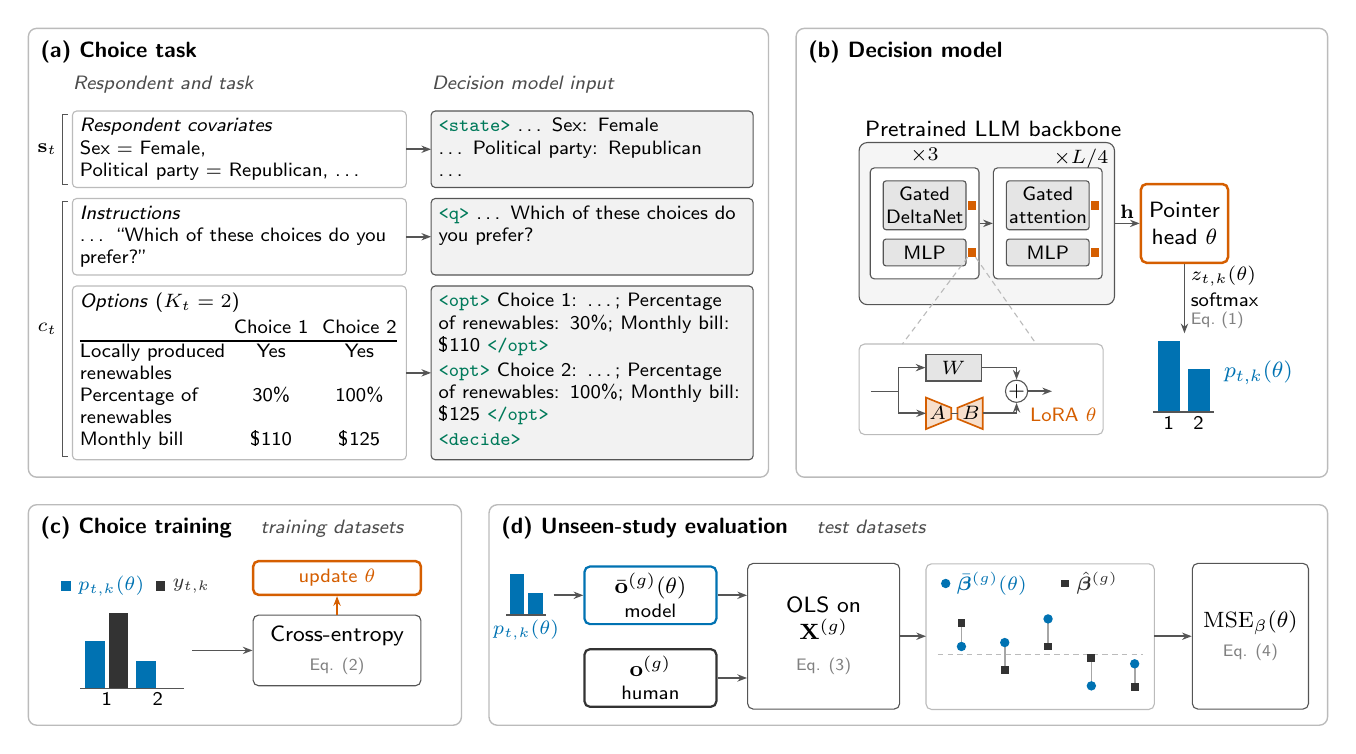
\begin{tikzpicture}

% ---------------------------------------------------------------- frames, titles, subtitles
\draw[panel] (0,0) rectangle (9.4,-5.7);
\draw[panel] (9.75,0) rectangle (16.5,-5.7);
\draw[panel] (0,-6.05) rectangle (5.5,-8.85);
\draw[panel] (5.85,-6.05) rectangle (16.5,-8.85);

\node[ptitle] at (0.15,-0.15) {(a) Choice task};
\node[ptitle] at (9.9,-0.15) {(b) Decision model};
\node[ptitle] (tc) at (0.15,-6.2) {(c) Choice training};
\node[ptitle] (td) at (6.0,-6.2) {(d) Unseen-study evaluation};
\node[note, font=\scriptsize\itshape, anchor=base west] at ($(tc.base east)+(0.35,0)$) {training datasets};
\node[note, font=\scriptsize\itshape, anchor=base west] at ($(td.base east)+(0.35,0)$) {test datasets};

\newcommand{\eqtag}[1]{\textcolor{black!50}{\fontsize{6}{7}\selectfont Eq.~(#1)}}

% ================================================================ (a)
\node[note, font=\scriptsize\itshape] at (0.56,-0.6) {Respondent and task};
\node[note, font=\scriptsize\itshape] at (5.12,-0.6) {Decision model input};

\coordinate (inx) at (7.16,0);
\node[rawtxt, text width=4.05cm, anchor=north west] (rs) at (0.56,-1.05) {%
  \textit{Respondent covariates}\\
  Sex = Female,\\ Political party = Republican, \ldots};
\node[fieldtxt, text width=3.9cm, anchor=north] (fs) at (rs.north -| inx) {%
  \tok{<state>} \ldots\ Sex: Female\\
  \ldots\ Political party: Republican\\
  \ldots};
\rowboxes{rs}{fs}{b1}

\node[rawtxt, text width=4.05cm, anchor=north west] (ri) at ($(b1)+(0.56,-0.14)$) {%
  \textit{Instructions}\\
  \ldots\ ``Which of these choices do you prefer?''};
\node[fieldtxt, text width=3.9cm, anchor=north] (fi) at (ri.north -| inx) {%
  \tok{<q>} \ldots\ Which of these choices do you prefer?};
\rowboxes{ri}{fi}{b2}

\node[rawtxt, text width=4.05cm, anchor=north west] (rc) at ($(b2)+(0.56,-0.14)$) {%
  \textit{Options} ($K_t = 2$)\\[1pt]
  \begin{tabular}{@{}>{\raggedright\arraybackslash}p{1.85cm}@{\hspace{3pt}}c@{\hspace{5pt}}c@{}}
                              & Choice 1 & Choice 2 \\ \hline
  Locally produced renewables & Yes   & Yes   \\
  Percentage of renewables    & 30\%  & 100\% \\
  Monthly bill                & \$110 & \$125 \\
  \end{tabular}};
\node[fieldtxt, text width=3.9cm, anchor=north] (fc) at (rc.north -| inx) {%
  \tok{<opt>} Choice 1: \ldots; Percentage of renewables: 30\%; Monthly bill: \$110 \tok{</opt>}\\[1pt]
  \tok{<opt>} Choice 2: \ldots; Percentage of renewables: 100\%; Monthly bill: \$125 \tok{</opt>}\\[1pt]
  \tok{<decide>}};
\rowboxes{rc}{fc}{b3}

% Left brackets mapping Demographics -> s_t and Instructions + Options -> c_t
\draw[cline, line width=0.5pt]
  ($(rs.north west)+(-0.06,-0.04)$) -- ++(-0.07,0) |- ($(rs.west |- b1)+(-0.06,0.04)$);
\node[font=\scriptsize, anchor=east, inner sep=1.5pt] at ($($(rs.north west)!0.5!(rs.west |- b1)$)+(-0.14,0)$) {$\mathbf{s}_t$};

\draw[cline, line width=0.5pt]
  ($(ri.north west)+(-0.06,-0.04)$) -- ++(-0.07,0) |- ($(rc.west |- b3)+(-0.06,0.04)$);
\node[font=\scriptsize, anchor=east, inner sep=1.5pt] at ($($(ri.north west)!0.5!(rc.west |- b3)$)+(-0.14,0)$) {$c_t$};

% ================================================================ (b)
% backbone -> pointer head in one row; the output drops below the head
\coordinate (bbtop) at (10.55,-1.45);
\tikzset{
  layerbox/.style={draw=cline, fill=white, rounded corners=1.5pt, inner sep=0pt},
  mixer/.style={draw=cline, fill=black!10, rounded corners=1pt, align=center, font=\scriptsize,
                text width=0.98cm, minimum height=0.62cm, inner sep=1pt},
  mlp/.style={draw=cline, fill=black!10, rounded corners=1pt, align=center, font=\scriptsize,
              text width=0.98cm, minimum height=0.34cm, inner sep=1pt},
}
\newcommand{\loratab}[1]{\fill[ctrain] ($(#1.east)+(0.015,-0.06)$) rectangle ($(#1.east)+(0.115,0.06)$);}

\node[mixer, anchor=north west] (m1) at ($(bbtop)+(0.3,-0.48)$) {Gated\\DeltaNet};
\node[mlp, below=3pt of m1] (f1) {MLP};
\node[mixer, anchor=north west] (m2) at ($(m1.north east)+(0.5,0)$) {Gated\\attention};
\node[mlp, below=3pt of m2] (f2) {MLP};
\foreach \n in {m1,f1,m2,f2} { \loratab{\n} }
\begin{scope}[on background layer]
  \node[layerbox, fit=(m1)(f1), inner sep=4.5pt] (L1) {};
  \node[layerbox, fit=(m2)(f2), inner sep=4.5pt] (L2) {};
\end{scope}
\draw[flow] (L1.east) -- (L2.west);
\coordinate (bbse) at ($(L2.south east)+(0.15,-0.32)$);
\begin{pgfonlayer}{back}
  \draw[draw=cline, fill=black!4, rounded corners=3pt] (bbtop) rectangle (bbse);
\end{pgfonlayer}
\node[font=\scriptsize, anchor=south, inner sep=1.5pt] at (L1.north) {$\times 3$};
\node[font=\scriptsize, anchor=north east, inner sep=2pt] at (bbtop -| bbse) {$\times L/4$};
\node[font=\footnotesize, anchor=south west, inner sep=2pt] at (bbtop) {Pretrained LLM backbone};
\coordinate (bbE) at (bbse |- L1.west);

\node[trainbox, text width=0.93cm, minimum height=1.0cm, anchor=west] (ph) at ($(bbE)+(0.32,0)$) {Pointer head $\theta$};
\draw[flow] (bbE) -- (ph.west) node[midway, above, font=\scriptsize, inner sep=1.5pt] {$\mathbf{h}$};

\draw[flow] (ph.south) -- ++(0,-0.88)
  node[pos=0.18, right, font=\scriptsize, inner sep=2pt] {$z_{t,k}(\theta)$}
  node[pos=0.68, right, font=\scriptsize, align=left, inner sep=2pt] {softmax\\[-1.5pt]\eqtag{1}};
\coordinate (pb) at ($(ph.south)+(-0.34,-1.88)$);
\foreach \i/\h/\lab in {0/0.9/1, 1/0.55/2} {
  \fill[cpred] ($(pb)+(0.38*\i,0)$) rectangle ($(pb)+(0.38*\i+0.28,\h)$);
  \node[font=\scriptsize, below, inner sep=1.5pt] at ($(pb)+(0.38*\i+0.14,0)$) {\lab};
}
\draw[cline, line width=0.4pt] ($(pb)+(-0.06,0)$) -- ($(pb)+(0.72,0)$);
\node[font=\footnotesize, text=cpred, anchor=west, inner sep=1pt] at ($(pb)+(0.8,0.5)$) {$p_{t,k}(\theta)$};

% LoRA zoom-in under the backbone: every linear map is W + BA
\coordinate (lc) at ($(bbtop |- bbse)+(0.05,-1.1)$);
\draw[draw=cframe, rounded corners=2pt] ($(lc)+(-0.05,0.6)$) rectangle ($(lc)+(3.05,-0.55)$);
\draw[cframe, dash pattern=on 2pt off 1.5pt] ($(f1.east)+(0.015,-0.06)$) -- ($(lc)+(0.5,0.6)$);
\draw[cframe, dash pattern=on 2pt off 1.5pt] ($(f1.east)+(0.115,-0.06)$) -- ($(lc)+(2.2,0.6)$);
\node[draw=cline, fill=black!10, minimum width=0.7cm, minimum height=0.34cm, inner sep=0pt, font=\scriptsize] (W)
  at ($(lc)+(1.15,0.3)$) {$W$};
\draw[draw=ctrain, fill=ctrain!20, line width=0.6pt] ($(lc)+(0.8,-0.08)$) -- ($(lc)+(1.12,-0.21)$) -- ($(lc)+(1.12,-0.35)$) -- ($(lc)+(0.8,-0.48)$) -- cycle;
\draw[draw=ctrain, fill=ctrain!20, line width=0.6pt] ($(lc)+(1.2,-0.21)$) -- ($(lc)+(1.52,-0.08)$) -- ($(lc)+(1.52,-0.48)$) -- ($(lc)+(1.2,-0.35)$) -- cycle;
\node[font=\scriptsize, inner sep=0pt] at ($(lc)+(0.95,-0.28)$) {$A$};
\node[font=\scriptsize, inner sep=0pt] at ($(lc)+(1.37,-0.28)$) {$B$};
\node[draw=cline, circle, inner sep=0pt, minimum size=0.22cm, font=\scriptsize] (plus) at ($(lc)+(1.95,0)$) {$+$};
\draw[cline, line width=0.5pt] ($(lc)+(0.1,0)$) -- ($(lc)+(0.45,0)$) coordinate (split);
\draw[flow] (split) |- (W.west);
\draw[flow] (split) |- ($(lc)+(0.8,-0.28)$);
\draw[cline, line width=0.5pt] ($(lc)+(1.12,-0.28)$) -- ($(lc)+(1.2,-0.28)$);
\draw[flow] (W.east) -| (plus.north);
\draw[flow] ($(lc)+(1.52,-0.28)$) -| (plus.south);
\draw[flow] (plus.east) -- ($(lc)+(2.4,0)$);
\node[font=\scriptsize, text=ctrain, anchor=west, inner sep=1pt] at ($(lc)+(2.08,-0.3)$) {LoRA $\theta$};

% ================================================================ (c)
% horizontal legend on top of the bar chart, matching the style of (d)
\fill[cpred] (0.42,-7.14) rectangle (0.54,-7.02);
\node[font=\scriptsize, text=cpred, anchor=west, inner sep=1pt] at (0.59,-7.08) {$p_{t,k}(\theta)$};
\fill[chuman] (1.62,-7.14) rectangle (1.74,-7.02);
\node[font=\scriptsize, text=chuman, anchor=west, inner sep=1pt] at (1.79,-7.08) {$y_{t,k}$};
% model p (blue) next to human one-hot y (dark) for the two options; illustrative values
\coordinate (cb) at (0.72,-8.38);
\foreach \k/\p/\y in {0/0.60/0.95, 1/0.35/0} {
  \fill[cpred]  ($(cb)+(0.65*\k,0)$)     rectangle ($(cb)+(0.65*\k+0.25,\p)$);
  \fill[chuman] ($(cb)+(0.65*\k+0.3,0)$) rectangle ($(cb)+(0.65*\k+0.55,\y)$);
}
\node[font=\scriptsize, below, inner sep=1.5pt] at ($(cb)+(0.275,0)$) {1};
\node[font=\scriptsize, below, inner sep=1.5pt] at ($(cb)+(0.925,0)$) {2};
\draw[cline, line width=0.4pt] ($(cb)+(-0.06,0)$) -- ($(cb)+(1.26,0)$);

\node[box, text width=1.85cm, inner sep=4pt] (ce) at (3.92,-7.90) {Cross-entropy\\[1pt]\eqtag{2}};
\draw[flow] ($(cb)+(1.36,0.48)$) -- (ce.west |- {$(cb)+(0,0.48)$});
\node[trainbox, font=\scriptsize, text=ctrain, text width=1.85cm, inner xsep=4pt, inner ysep=3pt] (upd) at (3.92,-6.98) {update $\theta$};
\draw[->, line width=0.8pt, draw=ctrain] (ce.north) -- (upd.south);

% ================================================================ (d)
% the p glyph opens (d): same blue bars and label that close (b)
\coordinate (gb) at (6.12,-7.45);
\fill[cpred] (gb) rectangle ($(gb)+(0.18,0.52)$);
\fill[cpred] ($(gb)+(0.23,0)$) rectangle ($(gb)+(0.41,0.28)$);
\draw[cline, line width=0.4pt] ($(gb)+(-0.05,0)$) -- ($(gb)+(0.46,0)$);
\node[font=\scriptsize, text=cpred, anchor=north, inner sep=1.5pt] at ($(gb)+(0.2,0)$) {$p_{t,k}(\theta)$};

\node[predbox, text width=1.5cm] (ob) at (7.9,-7.2) {$\bar{\mathbf{o}}^{(g)}(\theta)$\\[-1pt]{\scriptsize model}};
\node[humanbox, text width=1.5cm] (oh) at (7.9,-8.25) {$\mathbf{o}^{(g)}$\\[-1pt]{\scriptsize human}};
\draw[flow] ($(gb)+(0.55,0.25)$) -- (ob.west |- {$(gb)+(0,0.25)$});
\node[box, text width=1.65cm, inner sep=4pt, minimum height=1.85cm] (ols) at (10.1,-7.72) {OLS on $\mathbf{X}^{(g)}$\\[2pt]\eqtag{3}};
\node[box, text width=1.3cm, minimum height=1.85cm] (mse) at (15.52,-7.72) {$\mathrm{MSE}_\beta(\theta)$\\[1pt]\eqtag{4}};
\draw[flow] (ob.east) -- (ob.east -| ols.west);
\draw[flow] (oh.east) -- (oh.east -| ols.west);

% slope-by-slope comparison; illustrative values (cm from the zero line)
\draw[draw=cframe, fill=white, rounded corners=2pt] (11.4,-6.8) rectangle (14.3,-8.65);
\fill[cpred] (11.65,-7.05) circle (1.7pt);
\node[font=\scriptsize, text=cpred, anchor=west, inner sep=1pt] at (11.75,-7.05) {$\bar{\boldsymbol{\beta}}^{(g)}(\theta)$};
\fill[chuman] (13.12,-7.10) rectangle (13.22,-7.00);
\node[font=\scriptsize, text=chuman, anchor=west, inner sep=1pt] at (13.27,-7.05) {$\hat{\boldsymbol{\beta}}^{(g)}$};
\draw[cframe, dash pattern=on 2pt off 1.5pt] (11.55,-7.95) -- (14.15,-7.95);
\foreach \i/\bh/\bm in {0/0.40/0.10, 1/-0.20/0.15, 2/0.10/0.45, 3/-0.05/-0.40, 4/-0.42/-0.12} {
  \draw[black!35, line width=0.6pt] (11.85+0.55*\i,-7.95+\bh) -- (11.85+0.55*\i,-7.95+\bm);
  \fill[chuman] (11.80+0.55*\i,-8.00+\bh) rectangle (11.90+0.55*\i,-7.90+\bh);
  \fill[cpred] (11.85+0.55*\i,-7.95+\bm) circle (1.7pt);
}
\draw[flow] (ols.east) -- (11.4,0 |- ols.east);
\draw[flow] (14.3,0 |- mse.west) -- (mse.west);

\end{tikzpicture}
\end{document}
